\chapter{BACKGROUND}



\section{The Automatic Speech Recognition Task}\label{sec:background}
Speech recognition or automatic speech recognition (ASR) is the task of 
predicting the text, sentence, transcription, or sequence of characters 
for a corresponding speech recording.
The general approach of ASR is to first compute feature representations called \emph{speech features} from given audio data,
and then map the speech features to characters or other tokens such as wordpieces.



\subsection{Speech recognition data}
The first step of creating an ASR model is to prepare the data that is used for the model.
A single data entry for an ASR dataset is a speech recording (typically in waveform audio file format)
along with a corresponding text transcription of the words which are spoken.
We explain why the choice of dataset has a significant effect on the accuracy of ASR models.

\paragraph*{The amount of training data.} The more data that is available during training the better the ability
of the ASR model to generalize. A small dataset (with few unique voices) may lead to overfitting to the specific 
voices in the dataset.
\paragraph*{The difference between read and conversational speech.} Humans tend to pronounce their speech more clearly 
when reading text from a transcript, and recent ASR models can predict read speech very accurately \cite{jurafskyspeech}.
In contrast, accurately predicting conversational speech is still a major challenge in ASR.
\paragraph*{Tonal qualities for different accents.} The accent of the speaker, which depends on the gender, 
age and ethnicity of the speaker is another important factor to bare in mind. Generally, male speakers
have a lower pitch compared to female speakers. Similarly, adult voices are generally have a lower pitch
compared to children.
\paragraph*{The audio quality of speech recordings.} The position of the microphone, the quality of the microphone, 
the number of microphones available, and the presence of background noise contribute towards the quality of speech recordings.



\subsection{Speech features}
Computing speech features is useful because audio data consists of a one-dimensional array of integers that describe the
amplitude of the recorded sound wave for small time periods called \emph{samples} (see Figure~\ref{}). 
The issue is that mapping a sequence of amplitude measurements to a sequence of characters is impractical. 
A common technique used to compute speech features is to transform the audio data from the amplitude-time domain 
to the frequency-time domain, using the Fast Fourier Transform (FFT) algorithm \cite{cochran1967fast}, \cite{cooley1969fast}.
However, in this study we discuss a more recent feature extraction approach based on contrastive learning.



\section{wav2vec 2.0}
wav2vec 2.0 provides a framework for learning speech representations using unlabeled speech data.
wav2vec 2.0 can be applied to a variety of speech-related tasks such as speech recognition, speech translation,
and speech classification.
It has proved to be particularly useful in cases where a lot of unlabeled data is available, but not much labeled data is available.
The authors show that using just ten minutes of labeled data and pre-training
on $53$k hours of unlabeled data still achieves $4.8$/$8.2$ WER on the clean/other test sets of Librispeech~\cite{}.

The general two-step approach for using wav2vec 2.0 for any speech-related task is the following.
First train (or ``pre-train'') the wav2vec 2.0 model on a large corpus of unlabeled data, which
will give you a model that converts audio data into speech features.
After pre-training, fine-tune the wav2vec 2.0 model for speech recognition using a much smaller corpus of labeled data. 
Fine-tuning wav2vec 2.0 for speech recognition involves replacing the head of the pretrained model with
an appropriate loss function such as CTC.

The wav2vec 2.0 architecture is described by the network diagram in Figure~\ref{wav2vec2_architecture}.
There are three important components of the wav2vec 2.0 architecture:
the feature-encoder, the quantization module, and the context network.
The objective of wav2vec 2.0 becomes clear only after understanding each of the three
components. Thus, the way in which wav2vec 2.0 is trained is only explained after discussing
the three components in detail.

\begin{figure}
    \centering
    \captionsetup{justification=centering}
    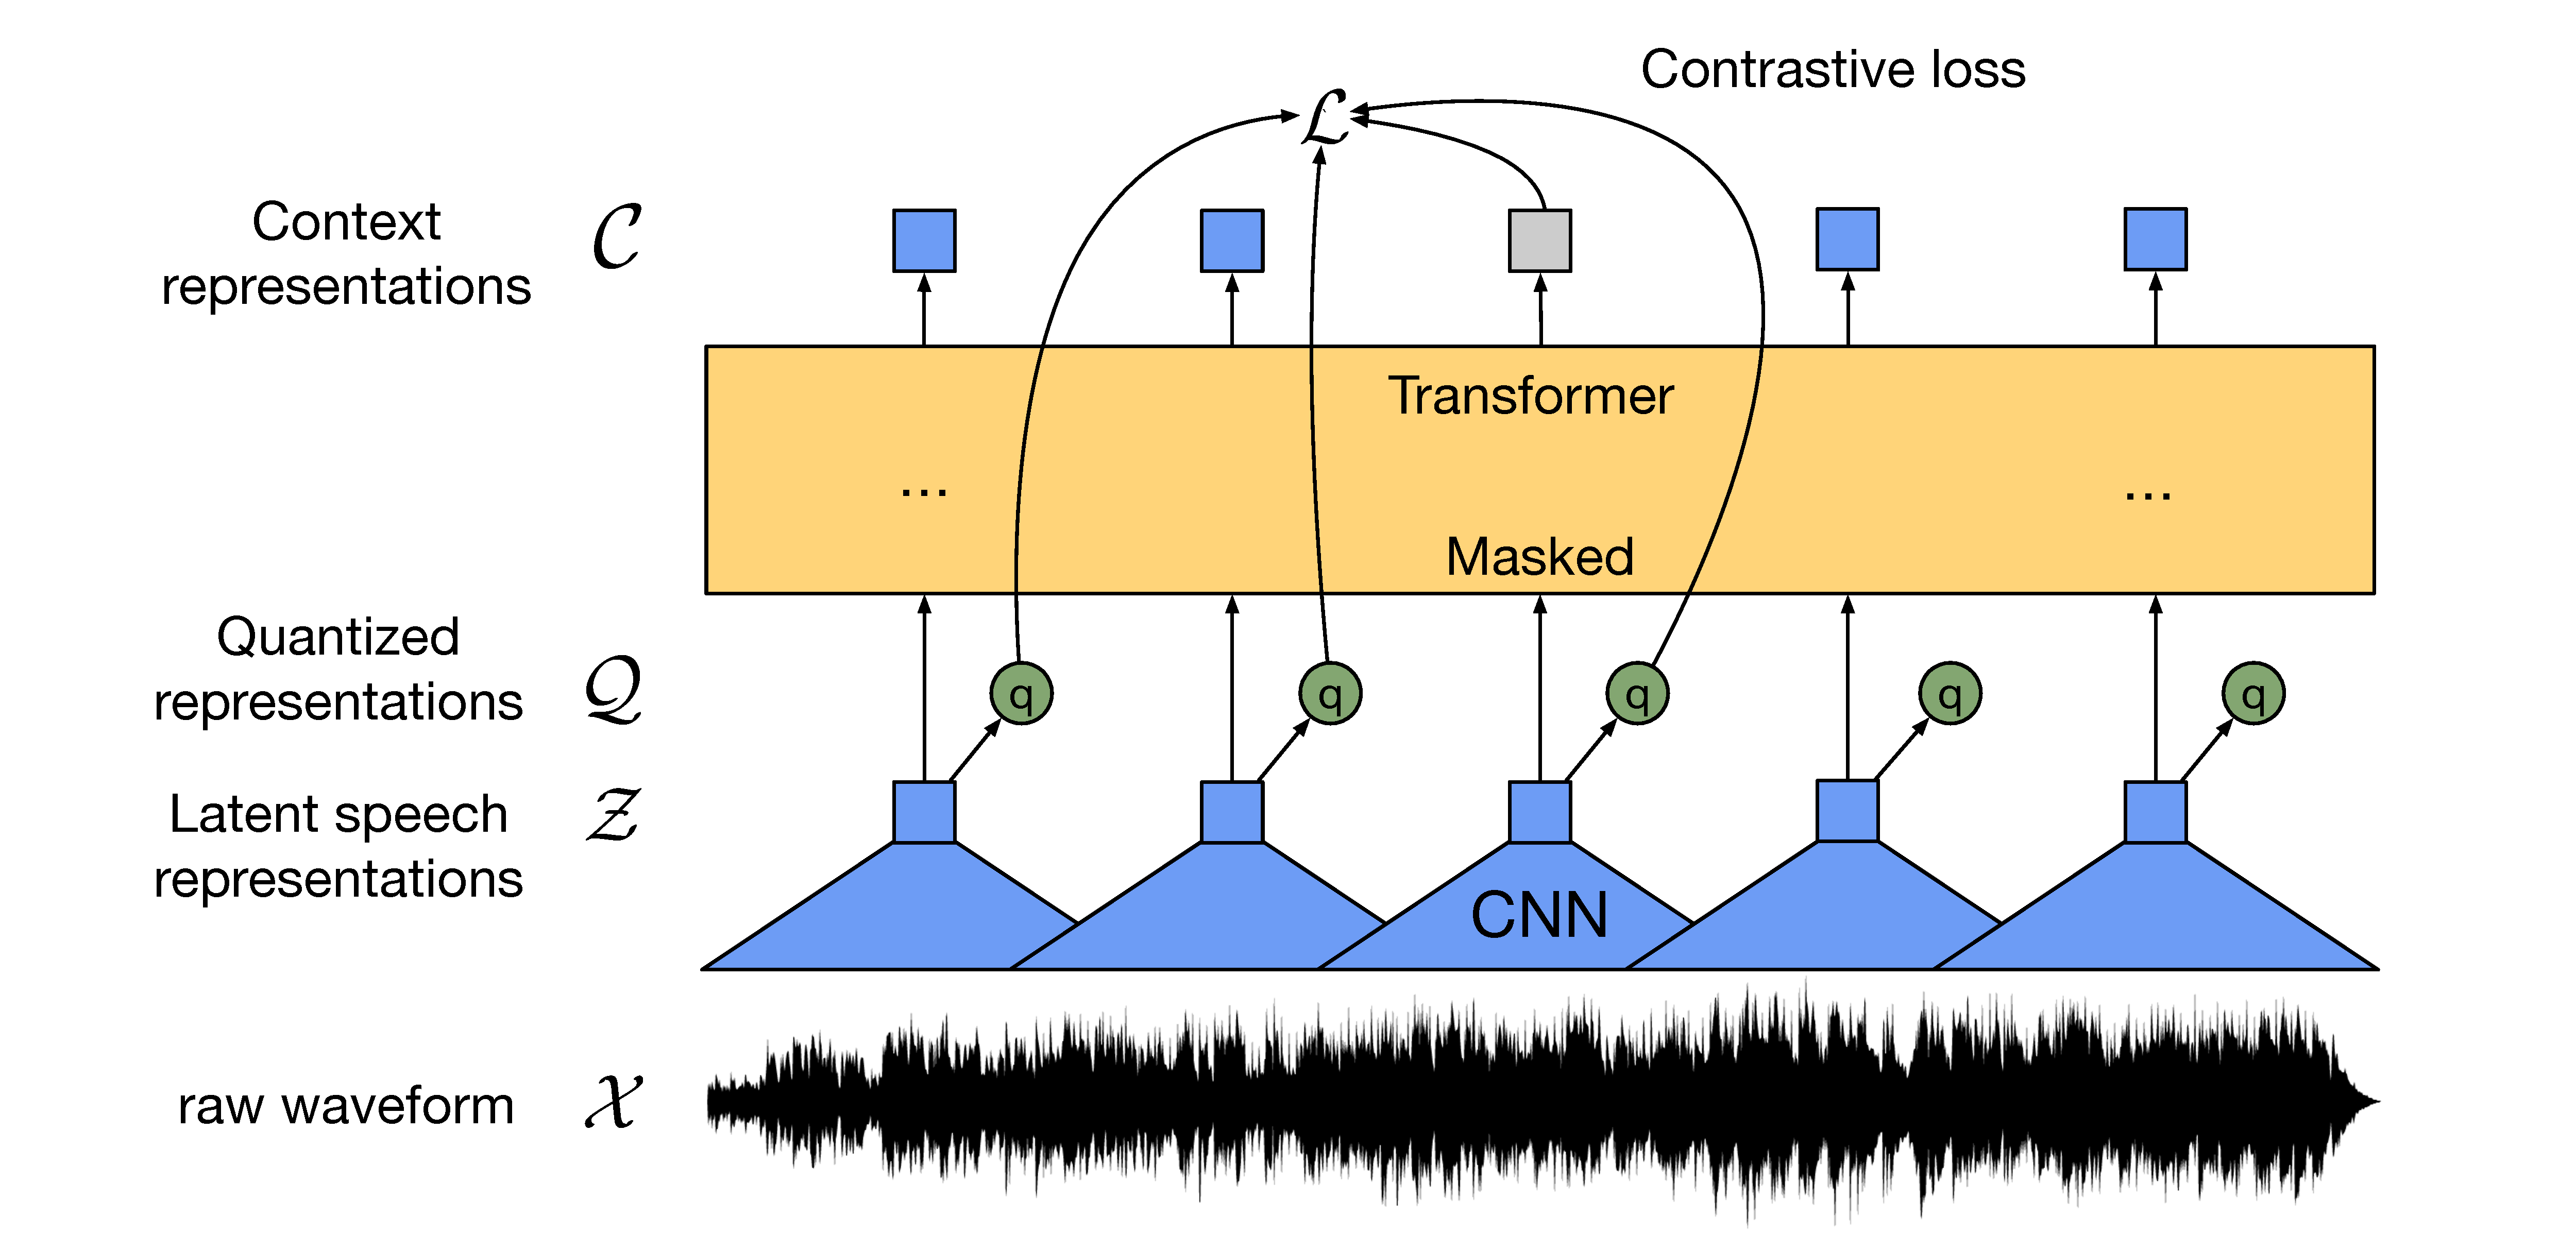
\includegraphics[width=\textwidth]{illustration.pdf}
    \caption{A visualization of the network architecture of wav2vec 2.0, taken from the original paper \cite{baevski2020wav2vec}.}
    \label{wav2vec2_architecture}
\end{figure}



\subsection{Feature encoder}
The feature encoder maps the raw audio data (speech recordings) to latent speech representations: $f: \mathcal{X} \rightarrow \mathcal{Z}$.
Thus, the feature encoder $f$ maps a sequence of audio samples $\mathbf{x}^{(1)}, \dots \mathbf{x}^{(N)}$ into a sequence of latent feature vectors $\mathbf{z}^{(1)}, \dots, \mathbf{z}^{(t)}$.
% Explain the purpose of feature encoder

The audio data is scaled to have zero mean and unit variance before going into the feature encoder. 
The feature encoder consists of seven convolutional blocks, where each convolutional block contains a temporal\footnote{One-dimensional convolutional layer designed for sequential data.} convolutional layer, 
a layer normalization layer, and the GELU activation function.

Each temporal convolutional layer contains 512 channels. 
The strides of the seven temporal convolutional layers are $(5,2,2,2,2,2,2)$ and the kernel widths are $(10,3,3,3,3,2,2)$.
The strides used results in each $\mathbf{z}^{(t)}$ representing $25$ms of audio (or $400$ input samples),
strided by about $20$ms.

Layer normalization scales the logits after each convolutional layer to have zero mean and unit variance, which has shown to increase the chances of earlier convergence.
GELU has become a popular activation function for NLP related tasks



\subsection{Quantization module}
The quantization module maps the latent speech features into discrete speech units: $h: \mathcal{Z} \rightarrow \mathcal{Q}$.
Speech is sound, and sound is represented as a continuous function. We would like to use Transformers and so continuous representations will not work. 
Unlike written language, which can be discretized into tokens such as characters or sub-words, speech does not have natural sub-units \cite{bgn2021illustrated}. 
The quantization module is a method in which discrete speech units are automatically learned using product quantization.

To perform product quantization, the quantization module uses $G$ \emph{codebooks}, where each codebook contains $V$ \emph{codebook entries} $\mathbf{e}_{1}, \dots, \mathbf{e}_{V}$.

The following steps describe the process of automatically assigning a discrete speech unit to each latent speech feature $\mathbf{z}^{(t)}$:
\begin{enumerate}
    \item Transform $\mathbf{z}^{(t)}$ into $\mathbf{l}^{(t)} \in \mathbb{R}^{G \times V}$ using a linear transformation.
    \item Choose one codebook entry $\mathbf{e}_g$ for each codebook $g = 1, \dots, G$, based on the values of $\mathbf{l}^{(t)}$.
    \item Concatenate the codebook entries $\mathbf{e}_1, \dots, \mathbf{e}_G$.
    \item Transform the resulting vector into $\mathbf{q}^{(t)} \in \mathbb{R}^{f}$ using another linear transformation.
\end{enumerate}
The two linear transformations are feed-forward neural networks $\text{FF}_1: \mathbb{R}^{f} \rightarrow \mathbb{R}^{G \times V}$ and $\text{FF}_2: \mathbb{R}^{d} \rightarrow \mathbb{R}^{f}$.
In the second step above, the codebook entry $\mathbf{e}_g$ is chosen as the one with the argmax of the logits $\mathbf{l}$. Choosing the codebook entries in this way is non-differentiable.
Fortunately, we can use the Gumbel softmax to choose codebook entries in a fully differentiable way. 
$\mathbf{e}_g$ is chosen as the entry that maximizes
\begin{equation}
    p_{g, v} = \dfrac{\exp{\left(\mathbf{l}^{(t)}_{g, v} + n_v\right)}/\tau}{\sum\limits_{k=1}^{V} \exp{\left(\mathbf{l}^{(t)}_{g, k} + n_k\right)}/\tau},
\end{equation}
where $\tau$ is a non-negative temperature, $n = -\log{(-\log{(u)})}$, and $u$ are uniform samples from $\mathcal{U}(0, 1)$.
During the forward pass, codeword $i$ is chosen by $i = \text{argmax}_j p_{g,j}$ and in the backward pass, the true gradient of the Gumbel softmax outputs is used.



\subsection{Context network}
% Explain what it is and its purpose
The context network creates contextualized representations from the feature encoder outputs.
The main component of the context network is a Transformer encoder \cite{transformer}.
Due to the popularity of Transformers we have ommited a detailed explanation of the Transformer architecture. 
Interested readers should refer to \cite{transformer} as well as guides such as \cite{alammar2018illustrated}.

% Explain architecture further
The following steps describe how the latent feature vectors are processed before being fed into the Transformer encoder.
\begin{enumerate}
    \item The latent feature vectors are fed into a \emph{feature projection layer} to match the model dimension of the context network.
    \item Positional embedding vectors are added to the inputs using \emph{relative positional encoding} \cite{shaw2018relative} instead of absolute positional encoding.
    The relative positional encoding is implemented using grouped convolution \cite{AlexNet}.
    \item Inputs are fed into the GELU activation function, followed by layer normalization.
\end{enumerate}

% Absolute position embeddings encode the absolute position of a word in the input phrase, the first word has position 1, 
% the 50th word has position 50. Relative position embeddings encode the relative position two words have to each other, 
% so the relative position between words 7 and 10 in a phrase would be 3.

% Explain LARGE Transformer encoder structure
The details for the Transformer encoder of the \textsc{LARGE} version of wav2vec 2.0 is as follows:
\begin{itemize}
    \item Numer of Transformer blocks: $B = 24$.
    \item Model dimension: $H_m = 1024$.
    \item Inner dimension: $H_{ff} = 4096$.
    \item Numer of attention heads: $A = 16$.
\end{itemize}



% \subsection{Objective function}
% % Talk about it
% There are two objectives (loss functions) that wav2vec 2.0 attempts to optimize simultaneously.
% The first loss function is the contrastive loss $\mathcal{L}_m$ which encourages the model to
% identify the true quantized representation for a masked time step within a set of distractors. 
% The second loss function is the diversity loss $\mathcal{L}_d$ which encourages the model 
% to equally use the codebook entries from the quantization module.

% \paragraph*{Contrastive loss.} 


% \paragraph*{Diversity loss.}
% % Do asap, get out of way



\subsection{Masking}

In Wav2Vec 2.0, the masking process plays a crucial role in pre-training. 
It involves two hyperparameters: $p = 0.065$ and $M = 10$. 
The masking is performed as follows:
\begin{enumerate}
    \item All time steps from the latent speech representation space $Z$ are considered.
    \item A proportion $p$ of vectors from the previous step is sampled without replacement. These sampled vectors determine the starting indices.
    \item For each starting index $i$, consecutive $M$ time steps are masked. There may be overlap between these masked spans.
\end{enumerate}

\subsection{Training Objective}

The training objective in Wav2Vec 2.0 consists of two main loss functions: contrastive loss ($L_m$) and diversity loss ($L_d$).

\subsubsection{Contrastive Loss ($L_m$)}

The contrastive loss is responsible for training the model to predict the correct quantized representation $q_t$ from a set of candidate representations $q' \in Q_t$. The set $Q_t$ includes the target $q_t$ and $K$ distractors sampled uniformly from other masked time steps. It is calculated as follows:

\begin{equation}
L_m = -\log \frac{\exp(\text{sim}(c_t, q_t) / \kappa)}{\sum_{q' \sim Q_t} \exp(\text{sim}(c_t, q') / \kappa)}
\end{equation}

Here, $\kappa$ represents a constant temperature, and $\text{sim}(a, b)$ denotes the cosine similarity between context representation $c_t$ and quantized representations $q$. This loss encourages the model to assign high similarity to the true positive target and penalize high similarity with negative distractors.

\subsubsection{Diversity Loss ($L_d$)}

The diversity loss is a regularization technique aimed at promoting the equal use of codebook entries. It is based on entropy and is calculated as:

\begin{equation}
L_d = -\sum_{g=1}^{G} \sum_{v=1}^{V} p̄_{g,v} \log p̄_{g,v}
\end{equation}

This loss maximizes the entropy of the softmax distribution $p̄_{g,v}$ over codebook entries, encouraging the model to utilize all code words equally.

\subsection{Pre-training and Contrastive Loss}

In the pre-training phase, a contrastive task is used to train the model on unlabeled speech data. A mask is randomly applied in the latent space, where approximately 50\% of the projected latent feature vectors are masked. These masked positions are replaced by the trained vector $Z'M$ before input to the Transformer network. The contrastive loss during pre-training encourages the model to differentiate between positive target representations and negative distractors.

\subsection{Diversity Loss during Pre-training}

To further ensure diversity in codebook usage, a diversity loss is added during pre-training. This loss maximizes the entropy of the softmax distribution over codebook entries, preventing the model from favoring a small sub-group of entries.

The overall training objective is a combination of contrastive loss and diversity loss, with a hyperparameter $\alpha$:

\begin{equation}
L = L_m + \alpha L_d
\end{equation}

where $\alpha$ is a tuned hyperparameter.



































\subsection{Fine-tuning}

\section{Connectionist Temporal Classification}
Connectionist Temporal Classification (CTC) \cite{graves2006connectionist} is an algorithm (or loss function) 
developed to map a sequence of speech features to a sequence of characters. The authors of the wav2vec 2.0 paper
suggest that if finetuning wav2vec 2.0 for ASR one should add a linear layer and CTC on top of the wav2vec 2.0 
network after pretraining on unlabeled audio data.



\subsection{Decoding with CTC}
% TODO: explain with diagram



\subsection{Improving performance with a language model}
% Write about $n$-gram models, Kneser-Nay, and stuff



\section{Finetuning pretrained wav2vec 2.0 models}
% TODO: Make sure what finetuning in my case means EXACTLY (which weights are frozen and which are not).
Pretraining on unlabeled audio data with wav2vec 2.0 is expensive and inconsistent.



\subsection{XLS-R}
% Talk about it